
%$$$$$$$$$$$$$$$$$$$$$$$$$$$$$$$$$$$$$$$$$$$$$$$$$$$$$$$$$$$$$$$$$$$$$$$$$$$$$$$$
%Paragraph 2:Concurrent updates에 대한 연구
%$$$$$$$$$$$$$$$$$$$$$$$$$$$$$$$$$$$$$$$$$$$$$$$$$$$$$$$$$$$$$$$$$$$$$$$$$$$$$$$$
\newpage
\section{확장성 있는 자료구조 연구}
\label{sec:datarelated}
%Many scalable data structures with scalable schemes show different performances
% depending on their update ratios.
많은 확장성 있는 방법과 사용되는 자료구조들은 업데이트 비율에 따라 다른 성능을 가진다.  
%In low and middle update rate, researchers have attempted to create new
% scalable schemes~\cite{McKenney98}~\cite{Matveev2015RLU}~\cite{Harris2001Lockfree}
%~\cite{Fomitchev2004Lockfree}
%~\cite{Timnat2012}
%or have attempted to adapt these scheme to data
%structures~\cite{Arbel2014ConcurrentRCU}~\cite{Dodds2015SCT}~\cite{AustinTClements2012RCUBalancedTrees}.
낮거나 중간 정도의 업데이트 비율에서는 연구자들은 새로운 확장성있는
기법~\cite{McKenney98}~\cite{Matveev2015RLU}~\cite{Harris2001Lockfree} ~\cite{Fomitchev2004Lockfree}
~\cite{Timnat2012}을 연구하거나 그 기법을 자료구조에 
적용~\cite{Arbel2014ConcurrentRCU}~\cite{Dodds2015SCT}~\cite{AustinTClements2012RCUBalancedTrees}을
하도록 시도하고 있다.
%In high update rate, the OpLog shows significant improvement in
%performance scalability for update-heavy data structures in
%many core systems, but suffers from limitation and overhead due
%to time-stamp counter management.
높은 업데이트 비율에서는 OpLog가 매니코어의 업데이트 비율이 높은 자료 구조에 대해서
 상당히 높은 성능 확장성을 가진다. 
%We substantially extend our preliminary work~\cite{Kyong2016LDU} not only to
% support per-core algorithm but also to apply the \LDU to anonymous rmap due to improving the
%Linux kernel scalability.

\subsection{확장성 있는 자료구조를 위한 동기화 기법}

\subsubsection{RCU}


확장성을 위한 대표적 동기화 기법인 RCU는 McKenney와 Slingwine에 의해 개발되었고, 
동기화 기법 때문에 발생하는 오버헤드를 최소화 시킨 방법이다.
특히 RCU는 리더들을 보호하기 위해 사용하는 동기화 기법의 오버헤드를 최소화 시킨다.
단점으로는 RCU의 라이터가 가 수행하는 방법은 복잡하고 느리다. 
이러한 단점에도 불구하고 리더들이 수행하는 락의 오버헤드가 적고, 여러 리더와 
업데이터 하나가 동시에 수행이 가능하므로 RCU는 현재 리눅스 커널에서 상당히 많이 사용되고 있다. 

\begin{figure}[h]
    \centering
    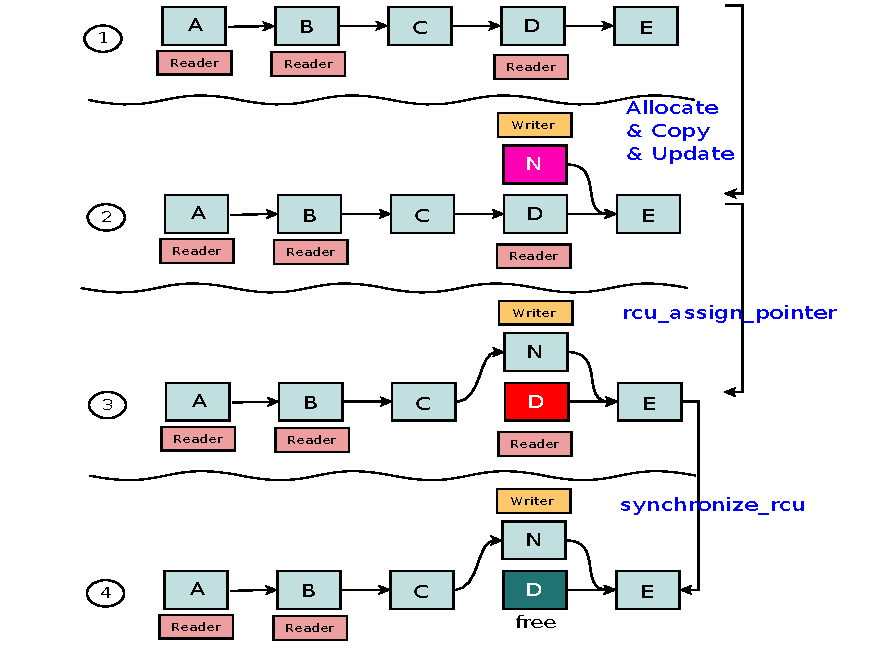
\includegraphics[width=1\textwidth]{fig/rcu/rcu_principle}
    \caption{RCU 예제}
  \label{fig:rcuprinciple}
\end{figure}

%$$$$$$$$$$$$$$$$$$$$$$$$$$$$$$$$$$$$$$$$$$$$$$$$$$$$$$$$$$$$$$$$$$$$$$$$$$$$$$$$
%Paragraph : RCU의 기본 철학
%$$$$$$$$$$$$$$$$$$$$$$$$$$$$$$$$$$$$$$$$$$$$$$$$$$$$$$$$$$$$$$$$$$$$$$$$$$$$$$$$
RCU의 기본 철학은 특정 시점에서 오브젝트를 복제해서 처리한다. 그림~\ref{fig:rcuprinciple}은 
이러한 RCU의 예를 보여준다.
그림에서 1단계에는 A, B, C, D, E 오브젝트 중 A, B, D 오브젝트를 리더들이 읽는 과정을 보여준다.
만약 이 순간 D 오브젝트를 수정하려 하면, RCU는 복사본을 할당 받고, 새로운 값인 오브젝트 N으로 수정을 한다.
그리고 다음 단계에서는 atomic한 연산을 통해서 오브젝트 C와 N을 연결한다. 
이 순간 오브젝트 D를 읽고 이는 리더와 다른 리더들은 아무런 블락 없이 계속 읽기를 수행할 수 있으며,
 동시에 업데이트까지 수행할 수 있어서 성능이 향상된다.
마지막으로 \code{synchroinze\_rcu()} 함수를 통해 리더가 읽기를 마칠 때 까지 기다리고, 읽기가 끝나면 
바로 \code{free()}를 수행한다. 
이 때 마지막 리더가 읽을 때 까지 기다리는 시간을 RCU에서는 grace period라 부른다. 

%$$$$$$$$$$$$$$$$$$$$$$$$$$$$$$$$$$$$$$$$$$$$$$$$$$$$$$$$$$$$$$$$$$$$$$$$$$$$$$$$
%Paragraph : RCU는 기본적으로 3가지 특징
%$$$$$$$$$$$$$$$$$$$$$$$$$$$$$$$$$$$$$$$$$$$$$$$$$$$$$$$$$$$$$$$$$$$$$$$$$$$$$$$$
RCU는 기본적으로 3가지 특징을 가진다. 첫 번째로 Lock-free 리더이다.
실제로 RCU의 리더들은 아무런 락 또는 배리어(barrier)를 소유하지 않고 수행되며, 리드 구간에서는
 per-core 자료구조에 단순히 enter/exit를 기록하여 수행한다. 
따라서, 락 발생하는 캐시 일관성 트래픽이 발생하지 않는다.
두번 째로, 싱글 포인터 업데이트이다.
RCU의 writer는 atomic 명령으로 one pointer 업데이트를 수행한다.
이러한 특징으로 인해 여러 리더들과 한가지 업데이터가 동시에 동작할 수 있다.  
마지막으로, RCU는 delayed free를 수행한다.
노드를 바로 free를 하지 않고, 모든 리더들이 리드 구역을 벋어난 경우 까지 
기다린 후 해당 노드를 free한다.
이를 통해 안전하게 노드를 자원 해재할 수 있다. 

\begin{figure}[h]
    \centering
    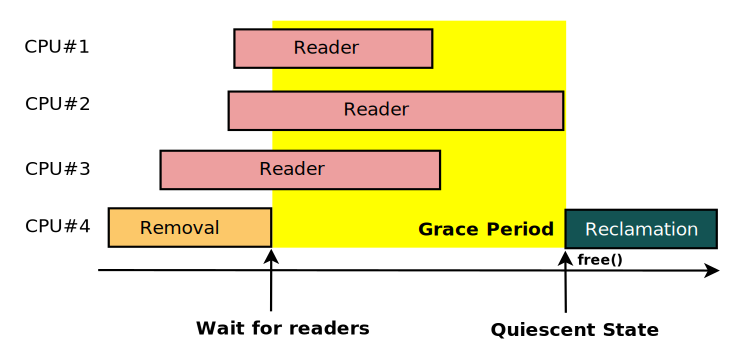
\includegraphics[width=1\textwidth]{fig/rcu/rcu_grace}
    \caption{RCU의 delayed free의 시점}
  \label{fig:rcu_grace}
\end{figure}

%$$$$$$$$$$$$$$$$$$$$$$$$$$$$$$$$$$$$$$$$$$$$$$$$$$$$$$$$$$$$$$$$$$$$$$$$$$$$$$$$
%Paragraph 2: RCU의 grace periad
%$$$$$$$$$$$$$$$$$$$$$$$$$$$$$$$$$$$$$$$$$$$$$$$$$$$$$$$$$$$$$$$$$$$$$$$$$$$$$$$$
그림~\ref{fig:rcu_grace}는 RCU의 delayed free의 시점을 보여준다.
RCU는 Removal 명령이 도착하면  Removal 명령을 수행하고 바로 \code{free()}를 수행하지 않는다. 
그 이유는 그 동안 해당 데이터는 리더들이 사용하고 있을 가능성이 있기 때문이다.
그 순간 부터 grace period 라고 부르는 리더들이 종료되기를 기다리고, quiescent state가 되면 
그 때 \code{free()}를 수행한다. 
현재는 리눅스 스케줄러에 의존하여 quiescent state를 판단하나, 
이러한  quiescent state를 마지막 리더가 끝나는 순간 바로 판단할 수 있는 방법들이 연구해야할 과제이다. 

\subsubsection{RLU}

%$$$$$$$$$$$$$$$$$$$$$$$$$$$$$$$$$$$$$$$$$$$$$$$$$$$$$$$$$$$$$$$$$$$$$$$$$$$$$$$$
%Paragraph : RLU가 해결하고자 하는 문제
%$$$$$$$$$$$$$$$$$$$$$$$$$$$$$$$$$$$$$$$$$$$$$$$$$$$$$$$$$$$$$$$$$$$$$$$$$$$$$$$$
RCU는 read-mostly 자료구조에 적합한 방법이나 
RCU는 사용하기에 프로그래머의 노력이 필요하고, 라이터들이 증가할 수록 많은 오버헤드를 가진다.
또한 RCU의 delayed free는 모든 리더가 종료했을 때 바로 quiescent state를 찾는 것이 아니기 때문에, 
이것음 암시적으로 시간에 민감한 응용프로그램에 문제를 가진다. 
이러한 문제를 해결하기 위해 만든것이 RLU~\cite{Matveev2015RLU}이다. 
RLU는 또 하나의 업데이트 문제를 해결한 
로그 기반 알고리즘이나, 이것은 read-mostly 자료구조에서 라이터의 원자적 명령어에 의한
오버헤드가 심한 문제를 싱글 원자적 명령어를 사용한 global clock 변수와 
오브젝트 레벨안에 per-core 단위로 로깅을 사용한 방법이다. 
따라서 업데이트가 많아지면 여전히 문제가 생긴다.


\subsubsection{Non-locking synchronization}

%$$$$$$$$$$$$$$$$$$$$$$$$$$$$$$$$$$$$$$$$$$$$$$$$$$$$$$$$$$$$$$$$$$$$$$$$$$$$$$$$
%Paragraph : Non-locking synchronization의 장점
%$$$$$$$$$$$$$$$$$$$$$$$$$$$$$$$$$$$$$$$$$$$$$$$$$$$$$$$$$$$$$$$$$$$$$$$$$$$$$$$$
Non-blocking synchronization은 장점은 여러 스레드들이 락 기반으로 자원을 관리함에 따라
 발생하는 문제를 해결할 수 있다. 
가장 큰 장점은 스레드 또는 프로세스가 락 때문에 기다리는 시간을 제거할 수 있다.
이 것은 락을 얻기 위해 기다리는 시간을 최소화 할 뿐만 아니라 무한 루프 때문에 무한정 기다리는 
데드락 같은 상황까지 제거 할 수 있다. 
다음으로 모든 락은 락 자체의 오버헤드를 가지고 있는데 이것을 제거할 수 있다. 
예를 들어 코어 수가 증가 할 수록 락 자체를 얻기 위해 원자적 명령을 이용한느데 이것은 캐시 일관성 트래픽을 
발생한다. 
이와 같이 Non-blocking 방법은 이러한 락 자체가 가지고 있는 문제점인 데드락(deadlock), 라이브락(livelock), 
우선순위 역전현상(priority inversion)등을 제거 할 수 있다. 
또한, Non-blocking synchronization 기법을 사용하는 lock-free 자료 구조들은 성능을 향상 시킬 수 있다. 
그 이유는 멀티코어 환경에서 공유되는 데이터를 접근하기 위해 직렬화 되는 부분이 매우 짧기 때문이다. 


\begin{figure}[h!]
    \centering
    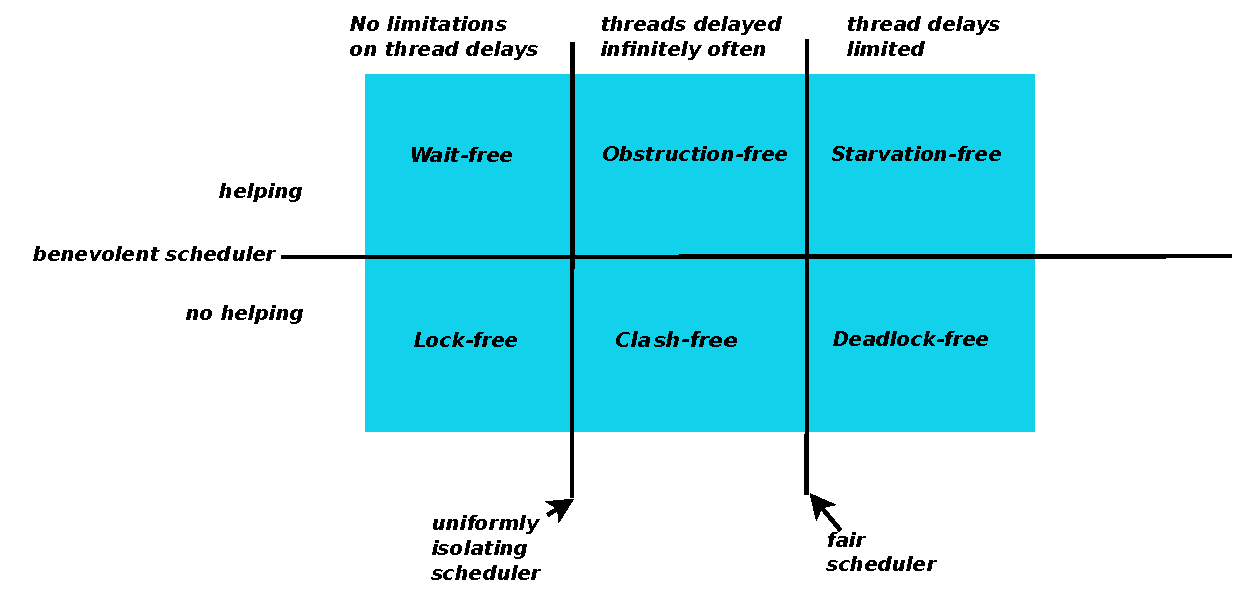
\includegraphics[width=1\textwidth]{fig/NBS/NBS}
    \caption{Non-locking 동기화 기법의 분류}
  \label{fig:NBS}
\end{figure}


%$$$$$$$$$$$$$$$$$$$$$$$$$$$$$$$$$$$$$$$$$$$$$$$$$$$$$$$$$$$$$$$$$$$$$$$$$$$$$$$$
%Paragraph : Non-locking synchronization 알고리즘 종류 1 
%$$$$$$$$$$$$$$$$$$$$$$$$$$$$$$$$$$$$$$$$$$$$$$$$$$$$$$$$$$$$$$$$$$$$$$$$$$$$$$$$
이러한 non-blocking 동기화 기법은 그림~\ref{fig:NBS}와 같이 분류된다.
크게 보면 \textit{Wait-free}방법과 \textit{Wait-free}으로 구분되고, 이것은 1990대 초에 
구분되었다.  
\textit{Wait-free} 방법은 가장 구현하기 힘든 알고리즘이며, 
모든 스레드가 딜레이 없이 바로 종료할 수 있는 알고리즘이다. 
다음으로 \textit{Lock-free} 방법은 적어도 하나의 스레드는 딜레이 없이 
바로 끝나는 방법이다. 
즉 그 이외의 스레드들은 전역 변수를 동시에 접근해서 발생하는 충돌 때문에 다시 
순회할 가능성이 있는 알고리즘이다.

\begin{figure}[h!]
\begin{center}
\inputminted[linenos,fontsize=\footnotesize,
tabsize=4]{c}{src/lockfree_stack.c}
\end{center}
\caption{간단한 Non-blocking 스택 알고리즘.}
\label{fig:nonblockingstack}
\end{figure}


%$$$$$$$$$$$$$$$$$$$$$$$$$$$$$$$$$$$$$$$$$$$$$$$$$$$$$$$$$$$$$$$$$$$$$$$$$$$$$$$$
%Paragraph : 심플 스택 알고리즘 설명
%$$$$$$$$$$$$$$$$$$$$$$$$$$$$$$$$$$$$$$$$$$$$$$$$$$$$$$$$$$$$$$$$$$$$$$$$$$$$$$$$
이러한 장점을 가진 Non-blockig Algortithm의 한 스택의 예는 그림 \ref{fig:nonblockingstack}과 같이
구현되어 있다.
자료구조의 내용은 value와 다음 노드를 가리키는 포인터가 존재한다(line 4).
\code{push} 함수 같은 경우를 보면, 먼저 새로운 노드에 스택의 top에 해당하는 노드를 저장(line 12)하고, 
CAS 연산을 통해 원자적으로 수정되었는지 체크를 함과 동시에 스택의 top에 해당하는 노드를 새로운 노드로 수정한다.
만약 CAS 연산이 실패하였다면(line 13), 즉 다른 스레드가 수정하였다면, 다시 처음부터 앞의 작업으로 
이동(line 11) 후 반복하여 수행한다.
\code{pop} 함수는 먼저 스택의 top에 해당하는 포인터를 지역 변수에 저장 후(line 20), CAS 연산을 통해 
원자적으로 top 다음 포인터를 가르키게 한 후(line 21) top에 해당하는 노드를 반환한다(line 23). 
만약 CAS 연산이 실패하며, \code{push} 처럼 반복 수행한다(line 19).

%$$$$$$$$$$$$$$$$$$$$$$$$$$$$$$$$$$$$$$$$$$$$$$$$$$$$$$$$$$$$$$$$$$$$$$$$$$$$$$$$
%Paragraph : ABA 문제 설명
%$$$$$$$$$$$$$$$$$$$$$$$$$$$$$$$$$$$$$$$$$$$$$$$$$$$$$$$$$$$$$$$$$$$$$$$$$$$$$$$$
Non-blocking synchronization의 가장 큰 현실적인 문제점은 바로 중간에 메모리를 재사용할 수 있기 때문이다.
예를 들어 스택에 \code{top->A->B->C}세가지 노드가 순차적으로 들어 있을 경우, 
CPU 1이 \code{CAS(top, A, B)} 명령어를 수행하고, 동시에 CPU 2가 A와 B를 꺼내고 A, B를 free한 후 
다시 A를 스택에 넣으면, CPU 1의 \code{CAS(top, A, B)} 명령어는 성공하게 되서, 
최종으로 \code{top->B->C} 이 스택에 쌓이게 되고, 처음과 다른 노드 A를 얻게 된다는 것이다.    
이러한 상황을 ABA 문제라고 한다. 
이러한 문제의 간단한 해결책은 \code{free()}를 바로 호출하지 않고, 
레퍼런스 카운트를 보고 해제하거나, 
안전한 시간(모든 프로세서가 작업이 끝날때)까지 기다린 후 호출하는 방법이 있다. 
 

\subsection{확장성 있는 자료구조}

\subsubsection{Harris Linked List}

%$$$$$$$$$$$$$$$$$$$$$$$$$$$$$$$$$$$$$$$$$$$$$$$$$$$$$$$$$$$$$$$$$$$$$$$$$$$$$$$$
%Paragraph 2: harris 알고리즘 설명
%$$$$$$$$$$$$$$$$$$$$$$$$$$$$$$$$$$$$$$$$$$$$$$$$$$$$$$$$$$$$$$$$$$$$$$$$$$$$$$$$
Non-blocking 알고리즘 중 대표적인 알고리즘 중 하나는 2001년도에 발표된 
Harris Linked List이다. 
Harris 알고리즘은 CAS를 이용한 알고리즘 중 하나이며, 순서대로 정렬된 노드들을 
순회하면서 해당 노드의 위치의 오른쪽 노드를 찾은 후 CAS로 해당 오른쪽 노드 앞에 새로운 노드를 삽입하는 방법이다.


\begin{figure}[h!]
    \centering
    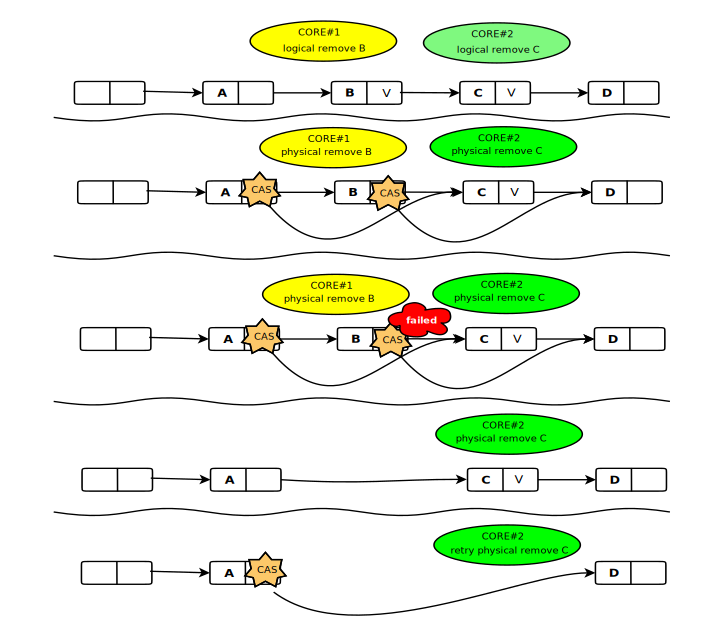
\includegraphics[width=1\textwidth]{fig/harris/harris}
    \caption{Harris 삭제}
  \label{fig:harris}
\end{figure}


%$$$$$$$$$$$$$$$$$$$$$$$$$$$$$$$$$$$$$$$$$$$$$$$$$$$$$$$$$$$$$$$$$$$$$$$$$$$$$$$$
%Paragraph 2: 그림 설명
%$$$$$$$$$$$$$$$$$$$$$$$$$$$$$$$$$$$$$$$$$$$$$$$$$$$$$$$$$$$$$$$$$$$$$$$$$$$$$$$$
그림~\ref{fig:harris}는 이러한 Harris 알고리즘 중 삭제하는 방법에 대해서 설명한다.
시간 순서 대로 위에서 아래로 진행된다.
제일 위에서는 동시에 \code{CORE1}이 노드 B를 삭제하고 \code{CORE2}가 노드 C를 삭제한다면,
Harris 링크드 리스트에서는 바로 삭제하지 않고 먼저 각 노드에 마킹을 한다. 
Harris 링크드 리스트 알고리즘에서는 이것을 \code{logical remove}라고 한다.
다음으로 \code{CORE1}과 \code{CORE2}가 동시에 CAS 연산으로 삭제를 하면, \code{CORE2}의 OLD 값이 
\code{CORE1}에 의해 변경되었기 때문에 이순간 CAS 실패가 발생하다. 
따라서 \code{logical remove}에 의해 논리적으로 제거는 되었지만 아직 노드가 남아 있는 상태가 된다.
Harris는 리스트는 CAS가 실패하면 처음 부터 다시 순회함으로 마킹된 노드를 제거하게 된다. 

%\subsubsection{Time-stamp stack}


